\documentclass{report}
\usepackage{graphics}
\usepackage{graphicx}

\title{Title of this Report}
\author {Author Name}

\begin{document}
\maketitle
\tableofcontents

\chapter{Introduction}

this is  a sample text.  this is  a sample text.  this is  a sample text.  this is  a sample text.  


this is  a sample text.
this is  a sample text.
this is  a sample text.
this is  a sample text.

\section{Earlier work} \label{ew}

this is  a sample text.
this is  a sample text.
this is  a sample text.
this is  a sample text.
this is  a sample text.

\section{Recent Work}

this is  a sample text.
this is  a sample text.
this is  a sample text.
this is  a sample text.
this is  a sample text.
this is  a sample text.

\section{Surveys in this area}

This is  a sample text.
this is  a sample text.
this is  a sample text.
this is  a sample text.
this is  a sample text.
this is  a sample text.
Approaches discussed Section in \ref{ew} do not include
the generic surverys.

This is  a sample text.
this is  a sample text.
this is  a sample text.
this is  a sample text.
this is  a sample text.
this is  a sample text.
this is  a sample text.
this is  a sample text.
this is  a sample text.
this is  a sample text.
this is  a sample text.
this is  a sample text as shown in Figure \ref{figsc}.

\begin{figure}
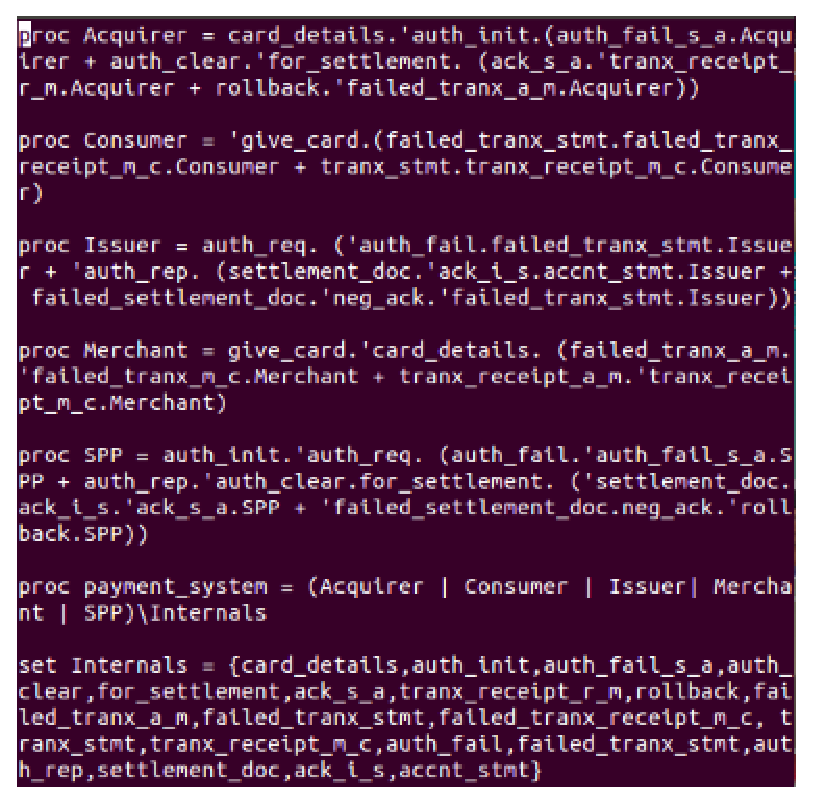
\includegraphics[width=7cm,height=2cm]{pics/pic1}
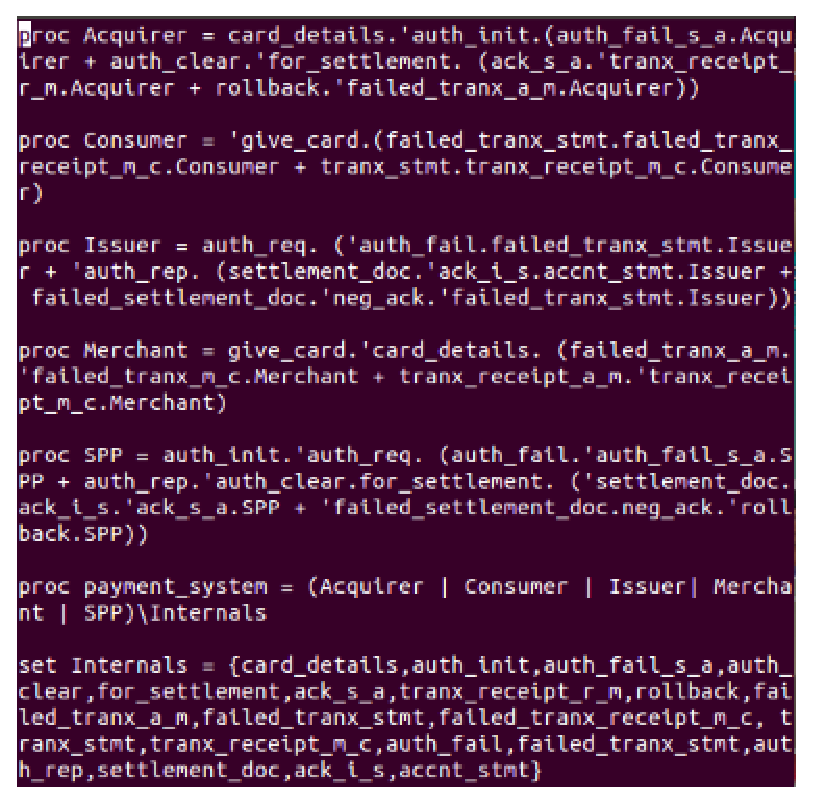
\includegraphics[scale=0.4]{pics/pic1}
\caption{A screenshot}
\label{figsc}
\end{figure}

\vspace{1mm}
\noindent
This is  a sample text.
this is  a sample text.
this is  a sample text.
this is  a sample text.
this is  a sample text \cite{Meyer2000}.
this is  a sample text \cite{Codishetal2000}.
this is  a sample text \cite{Huetal2000}.
this is  a sample text.
this is  a sample text.
this is  a sample text.
this is  a sample text.
this is  a sample text.


\chapter{Overview }

this is  a sample text.
this is  a sample text.
this is  a sample text.
this is  a sample text.

\begin{table}
\caption{Basic Data}
\begin{tabular} {|l|c|r|}
\hline
{\bf Name} & {bf Age} & {\bf Address} \\ \hline \hline
arima & 22 & New delhi somewhere in the lane\\
\hline
anok & 21 & TrichUr somewhere on a boat in the lake \\
\hline
\end{tabular}
\end{table}

this is  a sample text.
this is  a sample text.
this is  a sample text.
this is  a sample text.

\chapter{Mathematical formulation}

$\pi$ series by Ramanujan is as follows:

$\frac{1}{\pi} = \frac{\sqrt{8}}{9801} \times \sum\limits_{n=0}^{\infty} \times \frac{(4n)!}{(n!)^{4}} \times \frac{2390n+1103}{{396}^{4n}}$

$\overline{True} = False$ \\
$\underline{This \; is  \;important}$

\section{Equations with references}
\begin{equation} \label{eq}
 f(x) = x^{2} 
\end{equation}

The line defined by equation \ref{eq} is shown in the figure.

\section{Equation Arrays}

\begin{eqnarray}
a = b \\
c = d \times e
\end{eqnarray}

\chapter {Conclusions and Future Work}

These are the conclusions of my work.
These are the conclusions of my work.
These are the conclusions of my work.
These are the conclusions of my work.
These are the conclusions of my work.
These are the conclusions of my work.
These are the conclusions of my work.
These are the conclusions of my work.
These are the conclusions of my work.
These are the conclusions of my work.

These are the limitations.
These are the limitations.
These are the limitations.
These are the limitations.
These are the limitations.
These are the limitations.
These are the limitations.
These are the limitations.

In future these can be done.
In future these can be done.
In future these can be done.
In future these can be done.
In future these can be done.
In future these can be done.
In future these can be done.
In future these can be done.
In future these can be done.
In future these can be done.
In future these can be done.



\bibliographystyle{plain} 
\bibliography{myreferences}



\end{document}
